% Options for packages loaded elsewhere
\PassOptionsToPackage{unicode}{hyperref}
\PassOptionsToPackage{hyphens}{url}
%
\documentclass[
  12pt,
]{article}
\usepackage{lmodern}
\usepackage{amssymb,amsmath}
\usepackage{ifxetex,ifluatex}
\ifnum 0\ifxetex 1\fi\ifluatex 1\fi=0 % if pdftex
  \usepackage[T1]{fontenc}
  \usepackage[utf8]{inputenc}
  \usepackage{textcomp} % provide euro and other symbols
\else % if luatex or xetex
  \usepackage{unicode-math}
  \defaultfontfeatures{Scale=MatchLowercase}
  \defaultfontfeatures[\rmfamily]{Ligatures=TeX,Scale=1}
\fi
% Use upquote if available, for straight quotes in verbatim environments
\IfFileExists{upquote.sty}{\usepackage{upquote}}{}
\IfFileExists{microtype.sty}{% use microtype if available
  \usepackage[]{microtype}
  \UseMicrotypeSet[protrusion]{basicmath} % disable protrusion for tt fonts
}{}
\makeatletter
\@ifundefined{KOMAClassName}{% if non-KOMA class
  \IfFileExists{parskip.sty}{%
    \usepackage{parskip}
  }{% else
    \setlength{\parindent}{0pt}
    \setlength{\parskip}{6pt plus 2pt minus 1pt}}
}{% if KOMA class
  \KOMAoptions{parskip=half}}
\makeatother
\usepackage{xcolor}
\IfFileExists{xurl.sty}{\usepackage{xurl}}{} % add URL line breaks if available
\IfFileExists{bookmark.sty}{\usepackage{bookmark}}{\usepackage{hyperref}}
\hypersetup{
  pdftitle={Voting in a Pandemic --- COVID-19 and Primary Turnout in Milwaukee, Wisconsin},
  pdfauthor={Kevin Morris},
  hidelinks,
  pdfcreator={LaTeX via pandoc}}
\urlstyle{same} % disable monospaced font for URLs
\usepackage[margin=1in]{geometry}
\usepackage{longtable,booktabs}
% Correct order of tables after \paragraph or \subparagraph
\usepackage{etoolbox}
\makeatletter
\patchcmd\longtable{\par}{\if@noskipsec\mbox{}\fi\par}{}{}
\makeatother
% Allow footnotes in longtable head/foot
\IfFileExists{footnotehyper.sty}{\usepackage{footnotehyper}}{\usepackage{footnote}}
\makesavenoteenv{longtable}
\usepackage{graphicx}
\makeatletter
\def\maxwidth{\ifdim\Gin@nat@width>\linewidth\linewidth\else\Gin@nat@width\fi}
\def\maxheight{\ifdim\Gin@nat@height>\textheight\textheight\else\Gin@nat@height\fi}
\makeatother
% Scale images if necessary, so that they will not overflow the page
% margins by default, and it is still possible to overwrite the defaults
% using explicit options in \includegraphics[width, height, ...]{}
\setkeys{Gin}{width=\maxwidth,height=\maxheight,keepaspectratio}
% Set default figure placement to htbp
\makeatletter
\def\fps@figure{htbp}
\makeatother
\setlength{\emergencystretch}{3em} % prevent overfull lines
\providecommand{\tightlist}{%
  \setlength{\itemsep}{0pt}\setlength{\parskip}{0pt}}
\setcounter{secnumdepth}{5}
\usepackage{rotating}
\usepackage{setspace}
\usepackage{booktabs}
\usepackage{longtable}
\usepackage{array}
\usepackage{multirow}
\usepackage{wrapfig}
\usepackage{float}
\usepackage{colortbl}
\usepackage{pdflscape}
\usepackage{tabu}
\usepackage{threeparttable}
\usepackage{threeparttablex}
\usepackage[normalem]{ulem}
\usepackage{makecell}
\usepackage{xcolor}
\newlength{\cslhangindent}
\setlength{\cslhangindent}{1.5em}
\newenvironment{cslreferences}%
  {\setlength{\parindent}{0pt}%
  \everypar{\setlength{\hangindent}{\cslhangindent}}\ignorespaces}%
  {\par}

\title{Voting in a Pandemic --- COVID-19 and Primary Turnout in Milwaukee, Wisconsin}
\author{Kevin Morris\footnote{Researcher, Brennan Center for Justice at NYU School of Law, 120 Broadway Ste 1750, New York, NY 10271 (\href{mailto:kevin.morris@nyu.edu}{\nolinkurl{kevin.morris@nyu.edu}})}}
\date{June 09, 2020}

\begin{document}
\maketitle
\begin{abstract}
Abstract.
\end{abstract}

\pagenumbering{gobble}
\pagebreak

\pagenumbering{arabic}
\doublespacing

\hypertarget{data-and-research-design}{%
\section*{Data and Research Design}\label{data-and-research-design}}
\addcontentsline{toc}{section}{Data and Research Design}

We use individual-level voter registration and turnout records from L2 Political to estimate all our models. In addition to providing the information available in the registered voter file, L2 provides estimates for voters' race, household income, and education. L2 also geocodes voters to their home addresses.

Although Milwaukee, Wisconsin reduced their polling places from nearly 200 to just 5, the surrounding suburban municipalities did not see such drastic consolidation. However, residents of Milwaukee were also likely subject to a \emph{second} treatment: COVID-19 was apparently a worse crisis in Milwaukee City. In Milwaukee County there had been roughly 3.4 deaths per 10,000 residents attributed to COVID-19 as of June 8 according to data from the New York Times, compared with 2.4 deaths per 10,000 residents in Racine County, and 1.6, 0.8, and 0.7 in Ozaukee, Waukesha, and Washington Counties, respectively. Simply comparing the turnout of Milwaukee to the suburbs therefore cannot reveal the depressive effect of polling place consolidation alone, but rather the net effect of the worse health crisis and the consolidation.

To isolate the effect of polling place consolidation from the worse effects of COVID-19, we exploit the boundaries of the electoral jurisdictions to interrogate the effect of closing polling places on turnout in the April primary. Our primary design is therefore a regression discontinuity in space that exploits the municipal boundary line, comparing turnout for voters on either side of the ``cutpoint'' boundary. Here, we assume that voters who live in close proximity to one another but on either side of the adiminstrative boundaries were exposed to similar experiences with COVID-19; there is little reason to believe that COVID-19 operated differently on either side of an administrative boundary within a sufficiently narrow band.

The traditional regression discontinuity framework, however, relies on the assumption that individuals cannot ``select'' around the cutpoint; in other words, that within a narrow window individuals on either side of the cutpoint are identical. That is perhaps too strong of an assumption in this case; for instance, each suburban municipality bordering Milwaukee has its own school district. Voters very near one another but on opposite sides of the border might therefore differ in meaningful ways. Keele, Titiunik, and Zubizarreta (\protect\hyperlink{ref-Keele2015}{2015}) offers one way of dealing with this problem: ``When there appears to be strong self-selection around the border of interest, one alternative is to combine designs and to assume that, after conditioning on covariates, treatment assignment is as-if randomized for those who live near the city limit'' (page 228). This is the approach we take: we genetically match (Sekhon \protect\hyperlink{ref-Sekhon2011}{2011}) each registered voter in Milwaukee City (henceforth referred to as ``treated'' voters) to two voters who live outside the city but in Milwaukee, Racine, Waukesha, Washington, or Ozaukee County.\footnote{Each of these counties shares a border with the City of Milwaukee.} After the matching procedure has been completed, we test whether a treatment effect is present as we restrict the maximum distance allowed between treated and control voters.

Treated and control voters are matched \emph{exactly} on turnout in the 2016 and 2018 primary elections, and on their partisan affiliation. Voters are also matched on their gender, their household income, whether they have a collegiate education, and their race / ethnicity. Voters are also matched on their latitude and longitude to ensure physical proximity to one another. Although turnout is generally lower in the City of Milwaukee than in its suburbs, we account for this difference by the precise match on past turnout.

Although this differs from a regression discontinuity in which there is a band around a cutpoint, the logic is the same. As the maximum allowed distance between treated and control voters approaches zero, we are in fact reducing the band around the cutpoint represented by the municipal border. For instance, when the maximum distance allowed between a treated voter and her match is 150 feet, each voter will live (on average) 75 feet from the border. Conversely, by expanding the maximum allowed distance, we can estimate the net effect of polling place consolidation and the worse effects of COVID-19.

This set up allows us to test two hypotheses:

Hypothesis A: When the maximum distance allowed between treated and control voters approaches zero, voters in Milwaukee will have turned out at a lower rate than their controls just over the municipal border. This effect will be considered the effect of consolidated polling places.

Hypothesis B: As we allow the maximum allowed distance to increase, the negative treatment effect will grow larger. We expect that the worse effects of COVID-19 depressed turnout above-and-beyond the effects of consolidated polling places.

\hypertarget{results}{%
\section*{Results}\label{results}}
\addcontentsline{toc}{section}{Results}

We begin by presenting the results of the matching model, where each treated voter.\footnote{Due to computing constraints, we use a 1\% sample of voters (stratified by treatment status), though the whole pool is eventually used for the matching procedure itself.} Table \ref{tab:match} demonstrates that the matching procedure was largely successful: we achieve substantial improvement along all characteristics. It is perhaps worth noting that Milwaukee City is far less white; has far lower incomes and education levels; and saw much lower turnout in primary elections than suburban control voters. Although we do not include latitudes and longitudes in the balance table because they are largely uninterpretable, the average distance between a treated voter and her control is roughly 2 miles. Matching is done with replacement, and ties are not broken, which means that a treated might match with more than two controls; the regression weights are calculated accordingly.

\begin{singlespace}
\begin{table}[H]

\caption{\label{tab:balance-tab-chunk}\label{tab:match} Balance Table}
\centering
\resizebox{\linewidth}{!}{
\begin{tabular}[t]{lllllrrrr}
\toprule
\multicolumn{1}{c}{ } & \multicolumn{2}{c}{Means: Unmatched Data} & \multicolumn{2}{c}{Means: Matched Data} & \multicolumn{4}{c}{Percent Improvement} \\
\cmidrule(l{3pt}r{3pt}){2-3} \cmidrule(l{3pt}r{3pt}){4-5} \cmidrule(l{3pt}r{3pt}){6-9}
 & Treated & Control & Treated & Control & Mean Diff & eQQ Med & eQQ Mean & eQQ Max\\
\midrule
\% Voted in 2016 Primary & 27.0\% & 50.0\% & 27.0\% & 27.0\% & 100.00 & 100.00 & 100.00 & 100.00\\
\% Voted in 2018 Primary & 15.0\% & 27.0\% & 15.0\% & 15.0\% & 100.00 & 100.00 & 100.00 & 100.00\\
\% Male & 43.0\% & 45.0\% & 43.0\% & 43.0\% & 99.97 & 99.97 & 99.97 & 99.97\\
\% Democrats & 66.0\% & 25.0\% & 66.0\% & 66.0\% & 99.99 & 99.99 & 99.99 & 99.99\\
\% Republican & 9.0\% & 54.0\% & 9.0\% & 9.0\% & 100.00 & 100.00 & 100.00 & 100.00\\
Income & \$59,317 & \$96,615 & \$59,317 & \$59,330 & 99.96 & 99.96 & 99.92 & 99.83\\
\% with Collegiate Education & 13.0\% & 32.0\% & 13.0\% & 13.0\% & 100.00 & 100.00 & 100.00 & 100.00\\
\% White & 46.0\% & 75.0\% & 46.0\% & 46.0\% & 100.00 & 100.00 & 100.00 & 100.00\\
\% Black & 31.0\% & 2.0\% & 31.0\% & 31.0\% & 100.00 & 100.00 & 100.00 & 100.00\\
\% Latino & 9.0\% & 4.0\% & 9.0\% & 9.0\% & 100.00 & 100.00 & 100.00 & 100.00\\
\% Asian & 2.0\% & 2.0\% & 2.0\% & 2.0\% & 100.00 & 100.00 & 100.00 & 100.00\\
\bottomrule
\end{tabular}}
\end{table}
\end{singlespace}

Table \ref{tab:reg-table} presents the results of ordinary least squares regressions testing the treatment effect. In Table \ref{tab:reg-table} we require treated and control voters to live within 0.5 miles of one another.\footnote{A treated voter might live within the cutoff distance from one of her controls but not the other. The regression weights are updated for each regression to reflect this possibility.} The dependent variable takes the value 1 if a voter cast a ballot in the April primary, and 0 if she did not. We also test whether the treatment effect was different for Black voters than for other voters; research indicates that minority voters are both less likely to use vote-by-mail options and more likely to have their ballots rejecting, implying that the closed polling places might have decreased their turnout by even more than others'. Models 1 and 3 include just the treatment variable (and, in Model 3, the interaction terms) while Models 2 and 4 add in the variables on which the matching was performed (but without latitude and longitude). Robust standard errors are clustered at the level of the match (Abadie and Spiess \protect\hyperlink{ref-Abadie2019}{2019}).

\begin{singlespace}

\input{"../temp/reg.tex"}
\end{singlespace}

Models 1 and 2 indicate that turnout was depressed by roughly 8.6 percentage points in the April primary in Milwaukee City relative to suburban voters. Models 3 and 4 indicate that this decrease was especially pronounced among Black voters, who saw turnout nearly 10.2 percentage points below that of their suburban matches. Because of the tight geographic restriction imposed here, we argue that this represents the causal effect of polling place consolidation. This is a large treatment effect, and proves Hypothesis A correct.

We are also interested in whether the findings hold when we relax the geographic assumption by further restricting the maximum allowed distance, and also in whether the size of the treatment effect grows as we include pairs who live further away from one another. Figure \ref{fig:coef-plot} re-estimates of Model 3 from Table \ref{tab:reg-table} using different maximum distances between treated and control voters. When we restrict the pool to pairs who live within 0.25 miles, and within 150 feet, of one another, our overall treatment effect remains large and highly statistically significant, bolstering evidence of a treatment effect.

The interaction effect becomes non-significant, though it remains negative. This is probably due more to the fact that very few treated Black voters lived near the municipal border and had matches just on the other side; in our most conservative pool, we have just 82 treated Black voters, while Black voters make up just 5\% of the treated voters in the second-most-conservative model.

\begin{figure}[H]

{\centering 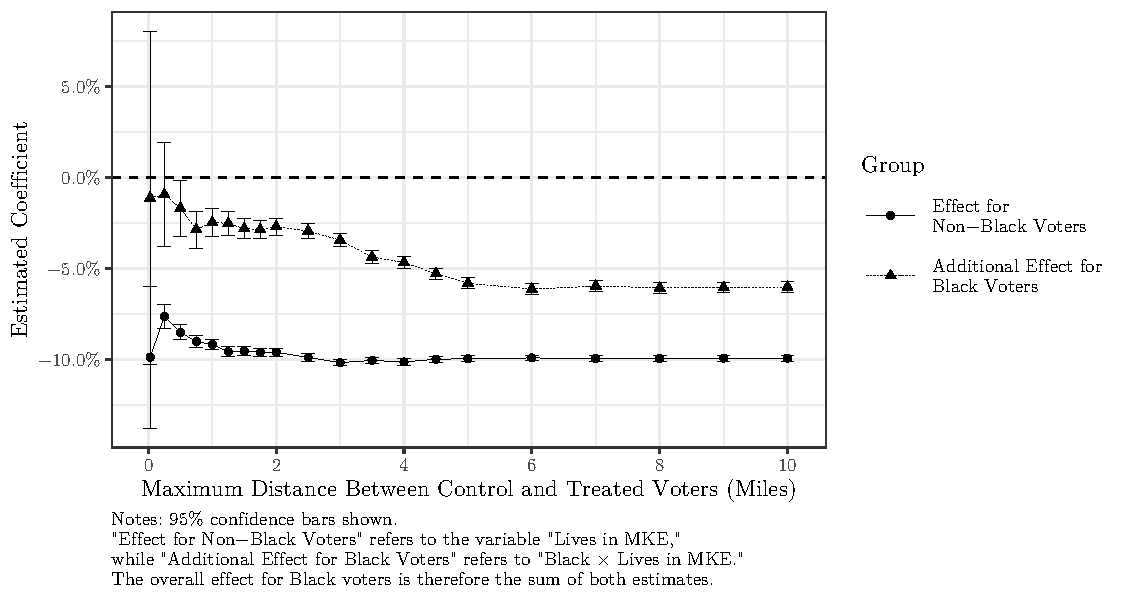
\includegraphics{markdown_files/figure-latex/plot-1} 

}

\caption{\label{fig:coef-plot}Estimated Depressive Effect of Living in MKE, 2020 Primary}\label{fig:plot}
\end{figure}

As we allow the maximum distance between treated and control voters to grow, the overall treatment effect and interaction effect become more negative; in other words, turnout in Milwaukee was apparently depressed by mechanisms above-and-beyond those explained by polling place consolidation and the voter demographics for which we controlled in the matching procedure. As discussed above, Milwaukee was hard-hit by the COVID-19 crisis; this analysis demonstrates that COVID-19 likely depressed turnout in Milwaukee City. The difference in overall treatment effect between the most half-mile and most lenient models is roughly 3.2 percentage points (the interaction effect grows by 4.4 percentage points). Thus COVID-19 likely reduced turnout relative to the suburbs through mechanisms other than polling place consolidation by more than 3 percentage points for non-Black voters, and as much as 7.6 percentage points for Black voters.

\newpage

\hypertarget{references}{%
\section*{References}\label{references}}
\addcontentsline{toc}{section}{References}

\hypertarget{refs}{}
\begin{cslreferences}
\leavevmode\hypertarget{ref-Abadie2019}{}%
Abadie, Alberto, and Jann Spiess. 2019. ``Robust Post-Matching Inference.'' \emph{Working Paper.}

\leavevmode\hypertarget{ref-Keele2015}{}%
Keele, Luke, Rocío Titiunik, and José R. Zubizarreta. 2015. ``Enhancing a Geographic Regression Discontinuity Design Through Matching to Estimate the Effect of Ballot Initiatives on Voter Turnout.'' \emph{Journal of the Royal Statistical Society: Series A (Statistics in Society)} 178 (1): 223--39. \url{https://doi.org/10.1111/rssa.12056}.

\leavevmode\hypertarget{ref-Sekhon2011}{}%
Sekhon, Jasjeet S. 2011. ``Multivariate and Propensity Score Matching Software with Automated Balance Optimization: The Matching Package for R.'' \emph{Journal of Statistical Software} 42 (1): 1--52. \url{https://doi.org/10.18637/jss.v042.i07}.
\end{cslreferences}

\end{document}
